\section{\thirdtitle}

\begin{frame}
\frametitle{\textbf{Patterns}}
  \begin{tabular}{p{5mm}p{90mm}}
    $b_{ip}$ &: aircraft $i$ uses check pattern $p$. \\
  \end{tabular}

  % TODO: this image
  % j and M => legend
  \DrawGantt{2}{2}{0}

\end{frame}

\begin{frame}
\frametitle{\textbf{Pattern representation}}
  % TODO: legend aircraft i, t, etc.
  % TODO: animation to explain a node, legend
  % TOOD: redo a simpler graph


\def\mydata{1, 2, 3, 4, 5, 6, 7, 8}

\foreach \x in \mydata
{
\pgfmathtruncatemacro\z{\x-1}
% \z{}
 \only<\x>{
    \begin{adjustbox}{max totalsize={\textwidth}{\textheight},center}
      \DrawGraph{\z}
   \end{adjustbox}
 }
}
  \only<1-2>{
  \DrawGantt{0}{0}{0}
  }
  \only<3>{
  \DrawGantt{1}{0}{0}
  }
  \only<4>{
  \DrawGantt{1}{0}{0}
  }
  \only<5>{
  \DrawGantt{1}{2}{0}
  }
  \only<6->{
  \DrawGantt{2}{2}{1}
  }
\end{frame}

\begin{frame}
\frametitle{\textbf{Pattern extraction}}
  % TODO: this

\end{frame}

\begin{frame}
\frametitle{\textbf{Solution approach}}
% TODO: animation
% TODO: size of End.
% TODO: arrows
\begin{adjustbox}{max totalsize={0.8\textwidth}{0.8\textheight},center}
        \begin{tikzpicture}
      [node distance=1.6cm,
      every node/.style={fill=white, font=\sffamily}, align=left]
     % Specification of nodes (position, etc.)
      \node (start)             [activityStarts]              {Start};

      % \onslide<+->{
        \node (initSol)     [startstop, below of=start]          {$x = getInitialSolution()$\\$z^* = \infty$\\$t = clock()$};
        \draw[->]             (start) -- (initSol);
      % }
      % \onslide<+->{
        \node (objFunc)      [master, below of=initSol]   {$err= getErrors(x)$\\$z=getObjective(x,err)$};
        \draw[->]     (initSol) -- (objFunc);
      % }
      % \onslide<+->{
         \node (maybeBest)      [master, below of=objFunc]   {$z < z^*$};
         \draw[->]     (objFunc) -- (maybeBest);
          \node (updateBest)      [master, right of=maybeBest, xshift=3cm]   {$x^* = x$\\$z^* = z$};
         \draw[->]      (maybeBest) -- node {Yes} (updateBest);
      % }
      % \onslide<+->{
        \node (maybeStop)      [master, below of=maybeBest, yshift=-0.5cm]   {$clock() -t > t_{max}$};
        \node (Stop)      [activityStarts, right of=maybeStop, xshift=3cm]   {End};
        \draw[->]     (maybeStop) -- node {Yes}  (Stop);
        \draw[->]      (maybeBest) -- node {No} (maybeStop);
        \draw[->]      (updateBest.south) -- ++(0,-.7) -- ++(-4.5,0)  -- (maybeStop.north);
      % }
      % \onslide<+->{
        \node (chooseNeighborFunc)     [master, below of=maybeStop, yshift=-0.5cm, neighborhoods]   {$move = choose\{S\hspace{-0.5mm}P\hspace{-0.5mm}A, RH\}$\\$\mathcal{T}_{c}, \mathcal{I}_{c} = getCandidate(err, move)$\\$x = move(x, \mathcal{T}_{c}, \mathcal{I}_{c})$};
        \draw[->] (chooseNeighborFunc.west) -- ++(-0.5,0) -- ++(0,3.8) -- ++(0,2) -- (objFunc.west);
        \draw[->]     (maybeStop) -- node {No} (chooseNeighborFunc);
      % }
 
      \end{tikzpicture}
\end{adjustbox}

\end{frame}

\begin{frame}
\frametitle{\textbf{Neighborhood 1: Shortest Path Algorithm (SPA)}}
% TODO: explain matrix, legend?

  \onslide<2->{
    $SPA(x, \mathcal{I}_c, \mathcal{T}_c)$
  }

  \onslide<3->{
    \begin{align*}
      A_{c} = \left(
      \begin{array}{*6{c}}
    1 & 1 & 1 & 1 & 0 & 0 \\
    \tikzmark{left}{0} & {\text -}1 & {\text -}1 & {\text -}1 & {\text -}1 & \tikzmark{right}{0} \\
    0 & 0 & 0 & 0 & 2 & 2 \\
    0 & 0 & 0 & 0 & 0 & 0
      \end{array}
      \right)
      \Highlight[first]
    \end{align*}
  }
  \onslide<4->{
    \begin{align*}
      A_{c+1} = \left(
      \begin{array}{*6{c}}
    1 & 1 & 1 & 1 & 0 & 0 \\
    \tikzmark{left}{0} & 1 & 1 & 1 & 2 & \tikzmark{right}{-1} \\
    0 & 0 & 0 & 0 & 2 & 2 \\
    0 & 0 & 0 & 0 & 0 & 0
      \end{array}
      \right)
    \Highlight[second]
  \end{align*}
  }
  \onslide<5->{
    \tikz[overlay,remember picture] {
      \draw[->,thick,red,dashed] (first.east) -- ++(2, -2)  node [right] {SPA} -- (second.east);
    }
  }

\end{frame}

\begin{frame}
\frametitle{\textbf{Neighborhood 2: Rolling Horizon (RH)}}
  
  \onslide<2->{
    $RH(x, \mathcal{I}_c, \mathcal{T}_c)$
  }
  \onslide<3->{
    \begin{align*}
      A_{c} = \left(
      \begin{array}{*6{c}}
        1 & \tikzmark{left}{1} & 1 & 1 & 0 & 0 \\
        {\text -}1 & 0 & 0 & 0 & 0 & {\text -}1 \\
        0 & 0 & 0 & \tikzmark{right}{0} & 2 & 2 \\
        0 & 0 & 0 & 0 & 0 & 0
      \end{array}
      \right)
      \Highlight[first]
    \end{align*}  
  }
  \onslide<4->{
    \begin{align*}
      A_{c+1} = \left(
      \begin{array}{*6{c}}
        1 & \tikzmark{left}{0} & 0 & 0 & 0 & 0 \\
        {\text -}1 & 0 & 0 & 0 & 0 & {\text -}1 \\
        0 & 1 & 1 & \tikzmark{right}{1} & 2 & 2 \\
        0 & 0 & 0 & 0 & 0 & 0
      \end{array}
      \right)
    \Highlight[second]
    \end{align*}
  }
  \onslide<5->{
    \tikz[overlay,remember picture] {
      \draw[->,thick,red,dashed] (first.east) -- ++(4, -2) node [right] {RH} -- (second.east);
    }
  }
\end{frame}

\begin{frame}
\frametitle{\textbf{Initial solution}}

  Three ways.\\
  $SPA(\varnothing, \mathcal{I}, \mathcal{T})$

    \only<2>{
      \begin{align*}
        \left(
        \begin{array}{*6{c}}
          0 & 0 & 0 & 0 & 0 & 0 \\
          0 & 0 & 0 & 0 & 0 & 0 \\
          0 & 0 & 0 & 0 & 0 & 0 \\
          0 & 0 & 0 & 0 & 0 & 0
        \end{array}
        \right)
    \end{align*}
    }
    \only<3>{
      \begin{align*}
        \left(
        \begin{array}{*6{c}}
          0 & 0 & 0 & 0 & 0 & 0 \\
          \tikzmark{left}{0} & 1 & 1 & 1 & 2 & \tikzmark{right}{-1} \\
          0 & 0 & 0 & 0 & 0 & 0 \\
          0 & 0 & 0 & 0 & 0 & 0
        \end{array}
        \right)
      \Highlight[second]
    \end{align*}
    }
    \only<4>{
      \begin{align*}
        \left(
        \begin{array}{*6{c}}
          \tikzmark{left}{1} & 1 & 1 & 1 & 0 & \tikzmark{right}{0} \\
          0 & 1 & 1 & 1 & 2 & {\text -}1 \\
          0 & 0 & 0 & 0 & 0 & 0 \\
          0 & 0 & 0 & 0 & 0 & 0
        \end{array}
        \right)
      \Highlight[second]
    \end{align*}
    }
    \only<5>{
      \begin{align*}
       \left(
        \begin{array}{*6{c}}
          1 & 1 & 1 & 1 & 0 & 0 \\
          0 & 1 & 1 & 1 & 2 & {\text -}1 \\
          \tikzmark{left}{0} & 0 & 0 & 0 & 2 & \tikzmark{right}{2} \\
          0 & 0 & 0 & 0 & 0 & 0
        \end{array}
        \right)
      \Highlight[second]
    \end{align*}
    }

  $RH(\varnothing, \mathcal{I}, \mathcal{T})$ \\
  \only<6>{
      \begin{align*}
        \left(
        \begin{array}{*6{c}}
          \tikzmark{left}{0} & 0 & 0 & 0 & 0 & 0 \\
          0 & 0 & 0 & 0 & 0 & 0 \\
          0 & 0 & 0 & 0 & 0 & 0 \\
          0 & 0 & 0 & 0 & 0 & \tikzmark{right}{0}
        \end{array}
        \right)
        \Highlight[first]
      \end{align*}
  }

    \only<7>{
      \begin{align*}
        \left(
        \begin{array}{*6{c}}
          \tikzmark{left}{1} & 1 & 1 & 1 & 0 & 0 \\
          0 & 1 & 1 & 1 & 2 & {\text -}1 \\
          0 & 0 & 0 & 0 & 2 & 2 \\
          0 & 0 & 0 & 0 & 0 & \tikzmark{right}{0}
        \end{array}
        \right)
      \Highlight[second]
    \end{align*}
    }
  maintFirst()

\end{frame}

\begin{frame}
\frametitle{\textbf{Experiments}}
  
  \begin{itemize}[<+->]

  \item Instance sizes: large ($I$=60), very large ($I$=100) and very-very large ($I$=255).
  \item CPLEX running 1 thread.
  \item Time limit at 20 minutes.
  \item 1 graph per cluster of aircraft and node aggregation with respect to remaining flight time1.
  \end{itemize}

  \pause

  All instances have 90 periods.
\end{frame}

\begin{frame}
\frametitle{\textbf{Results: comparing neighborhoods}}
  % TODO: VND = RH + SPA
  % TODO: Time in units
  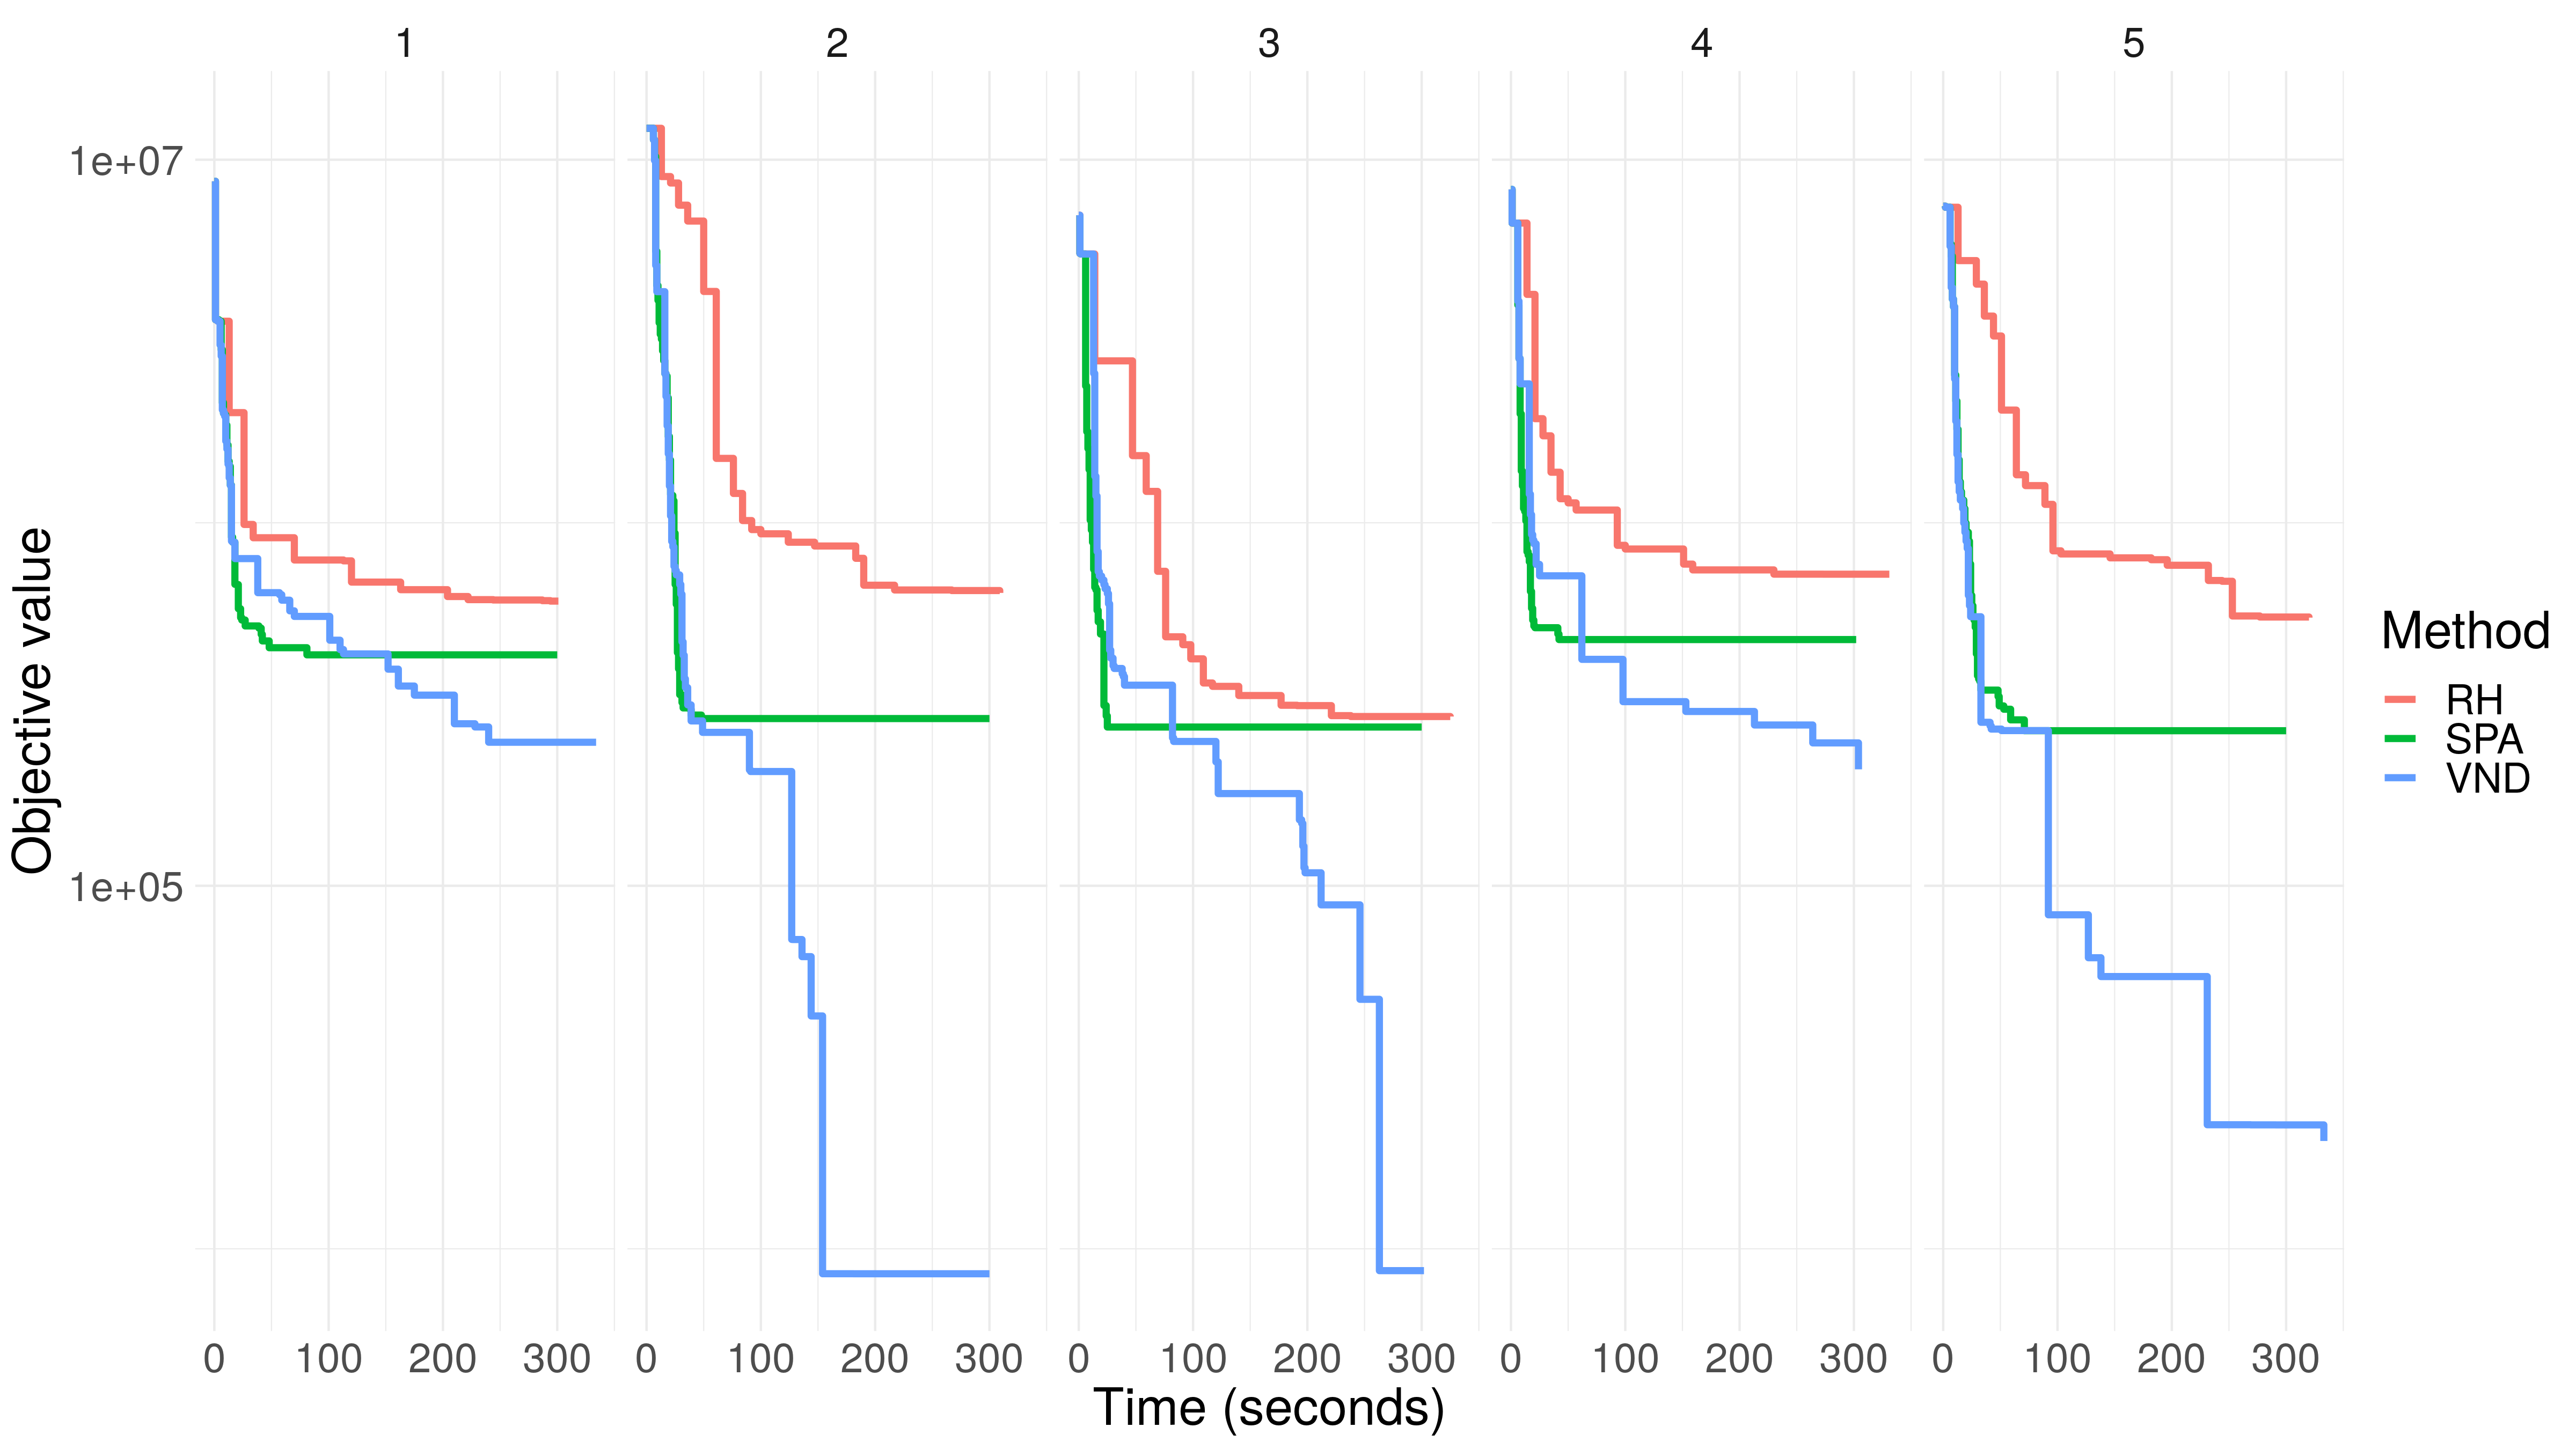
\includegraphics[width=\linewidth]{images/compare_neighbors.png}
\end{frame}

\begin{frame}
\frametitle{\textbf{Results: large instances}}
  % TODO: Time in units
  % TODO: size of police
  % TODO: rename instances
  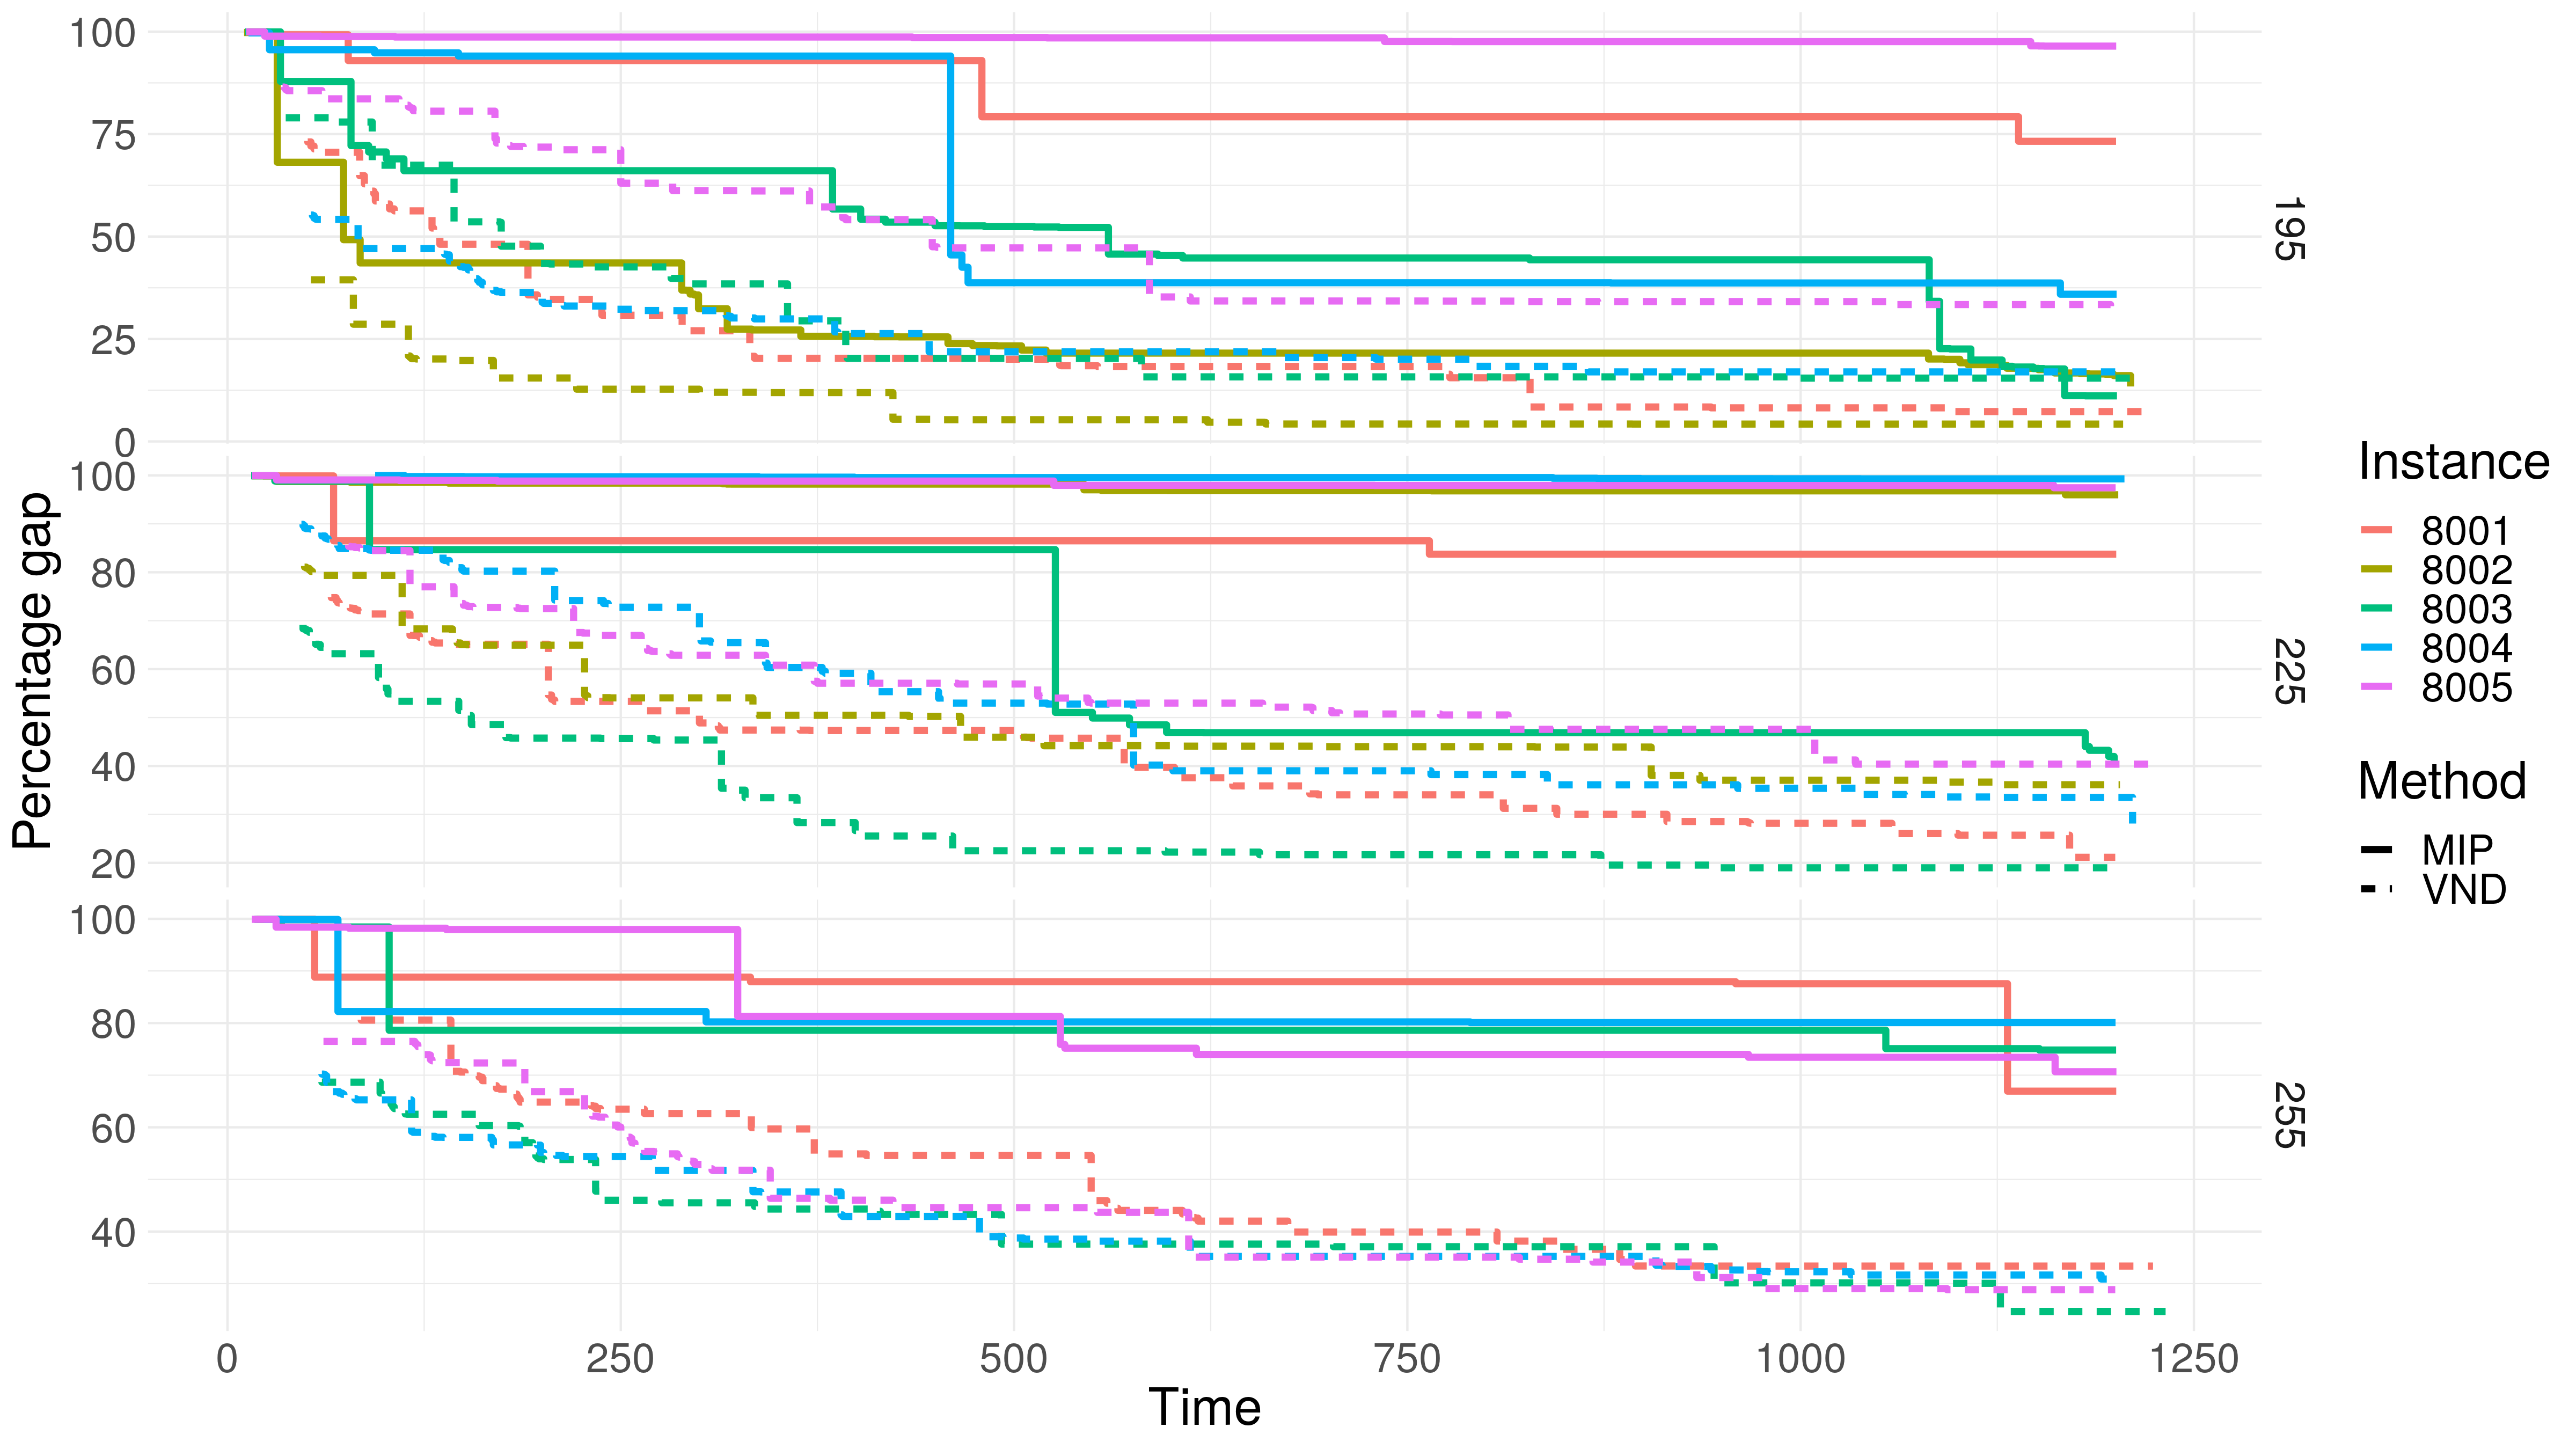
\includegraphics[width=\linewidth]{images/progress_gaps_very_large_255.png}  
\end{frame}

\begin{frame}
\frametitle{\textbf{Preliminary conclusions}}
  % TODO: check phrases
  % TODO: FMP and NRP: long?
  \pause
  \begin{block}{\textbf{Conclusions}}
    \begin{itemize}[<+->]
    \item \textbf{Graph representation} 
      built to efficiently explore the solution space of an aircraft.
    \item \textbf{Complementary neighborhoods} 
      are combined to efficiently explore the solution space.
    \end{itemize}
  \end{block}  
  \pause
  \begin{block}{\textbf{Perspectives}}
    \begin{itemize}[<+->]
      \item \textbf{Replace ad-hoc RH}
        e.g., by predicting / sampling promising patterns and running a set-covering model.
      \item \textbf{Apply graph in GRASP}
        by sampling paths in graph to quickly build solutions.
      \item \textbf{Generalize methodology}
        use it for the civil FMP problem or NRP.
    \end{itemize}
  \end{block}  
  
\end{frame}

